% main_report.tex
% 8CM00 Systems Medicine — Module 1 Group Assignment 3
% Compile with: pdflatex main_report.tex (x2 for references)

\documentclass[11pt, a4paper]{article}

% ---- Packages ----
\usepackage[utf8]{inputenc}
\usepackage[T1]{fontenc}
\usepackage{lmodern}
\usepackage[margin=2.5cm, headheight=14pt]{geometry}
\usepackage{amsmath, amssymb}
\usepackage{graphicx}
\usepackage{grffile}

% Safe image inclusion: shows placeholder if file is missing
\newcommand{\includefigure}[2][width=\textwidth]{%
  \IfFileExists{#2}{%
    \includegraphics[#1]{#2}%
  }{%
    \fbox{\parbox[c][4cm]{0.8\textwidth}{\centering\textit{Image not yet generated:}\\[0.5em]\detokenize{#2}}}%
  }%
}
\usepackage{booktabs}
\usepackage{caption}
\usepackage{subcaption}
\usepackage{hyperref}
\usepackage{xcolor}
\usepackage{float}
\usepackage{enumitem}
\usepackage{listings}
\usepackage{fancyhdr}
\usepackage{natbib}
\usepackage{parskip}              % spacing between paragraphs instead of indent
\usepackage[section]{placeins}    % keep floats within their section

% ---- Code listing style (MATLAB) ----
\lstset{
    language=Matlab,
    basicstyle=\ttfamily\footnotesize,
    keywordstyle=\color{blue},
    commentstyle=\color{gray},
    stringstyle=\color{orange},
    numbers=left,
    numberstyle=\tiny\color{gray},
    numbersep=5pt,
    frame=single,
    breaklines=true,
    captionpos=b,
    tabsize=4
}

% ---- Header/footer ----
\pagestyle{fancy}
\fancyhf{}
\lhead{8CM00 — Module 1 Assignment 3}
\rhead{Group 08}
\cfoot{\thepage}

% ---- Hyperlink style ----
\hypersetup{
    colorlinks=true,
    linkcolor=blue!60!black,
    citecolor=green!50!black,
    urlcolor=blue!70!black
}

% ---- Custom commands ----
\newcommand{\todo}[1]{\textcolor{red}{\textbf{[TODO: #1]}}}
\newcommand{\rxn}[1]{\texttt{#1}}          % reaction IDs in monospace
\newcommand{\gene}[1]{\textit{#1}}         % gene names in italics

% ============================================================================
\begin{document}

% ---- Title ----
\begin{titlepage}
\centering
\vspace*{3cm}
{\LARGE\bfseries 8CM00 Systems Medicine\\[0.3cm]
Module 1 — Group Assignment 3\par}
\vspace{1.5cm}
{\Large Genome-Scale Metabolic Modelling of\\
Adipose Tissue Under Caloric Restriction\par}
\vspace{2cm}
{\large
\begin{tabular}{ll}
    \textbf{Student 1:} & Tingan Kuo — 1758128 \\
    \textbf{Student 2:} & Gabriele Salvo — 2140004 \\
\end{tabular}
\par}
\vspace{1.5cm}
{\large Eindhoven University of Technology\\
Department of Biomedical Engineering\par}
\vspace{1cm}
{\large \today\par}
\vfill
\end{titlepage}

% ---- Table of Contents ----
\tableofcontents
\newpage

% ============================================================================
\section{Introduction}
\label{sec:intro}

Adipose tissue plays a dual role as an energy store and a paracrine organ, producing hormones such as leptin and adiponectin that regulate whole-body energy homeostasis. In obesity, rapid adipose expansion can outpace angiogenesis, leading to hypoxia, macrophage infiltration, and chronic inflammation that impairs metabolic function. While caloric restriction reduces adipose mass, previously obesogenic adipocytes retain a metabolic ``memory'' that predisposes to weight regain, which is the so-called yoyo effect \citep{vink2017}.

In this report, we use genome-scale metabolic models (GSMMs) to investigate how acute caloric restriction impacts adipose tissue metabolism, using transcriptomic data from the Yoyo study \citep{vink2017}. We generate context-specific metabolic reconstructions using iMAT, compare model structures via Jaccard similarity, and analyse predicted flux distributions using flux balance analysis (FBA) and cosine similarity.

% ============================================================================
\section{Question 1: PCA of Whole-Genome Expression Data}
\label{sec:q1}
\subsection{PCA analysis}
PCA was applied to the whole genome adipose tissue gene expression dataset in order to explore the main sources of variability across the samples. The first principal component (PC1) explains $16.41\%$ of the total variance, while the second principal component (PC2) explains $13.01\%$ of the variance. Together, these two components capture $29.42\%$ of the total variation in the dataset. This indicates that gene expression variability is distributed across many dimensions, which is typical for high dimensional transcriptomic data where thousands of genes contribute to variation across individuals.

\subsection{Cluster analysis between baseline and post-intervention samples}
After we coloured the samples with baseline and post-intervention status, no clear separation between the two groups is observed, as shown in Figure~\ref{fig:q1_1}. Baseline and post-diet samples largely overlap in the PCA space, suggesting that the global gene expression profile of adipose tissue does not undergo a strong shift after the dietary intervention. While a few sample appear as outliers along PC1 or PC2, these do not form consistent clusters corresponding to intervention status.

\subsection{Cluster analysis between LCD and VLCD group}
Colouring the PCA by diet group (LCD vs VLCD) also does not reveal a clear separation between groups, as shown in Figure~\ref{fig:q1_2}. Samples from both diet interventions are intermingled across the PCA plot, indicating that the differences between individuals are larger than the differences between the two diet regimes at the whole genome expression level. This suggests that global transcriptional changes induced by LCD and VLCD may be subtle or restricted to specific gene sets rather than dominating the overall variance.

\subsection{PCA analysis of yoyo dataset}
Additionally, we looked into yoyo dataset. By colouring the samples with baseline BMI, it shows a gradient of BMI values across the PCA space, as shown in Figure~\ref{fig:q1_3}. However, no obvious trend or directional structure along either principal component. Similarly, when the samples are coloured by sex, male and female samples overlap substantially without forming distinct clusters, as shown in Figure~\ref{fig:q1_4}. These observations suggest that sex and BMI are not the primary drivers of the largest variance components in the dataset.

\begin{figure}[H]
\centering

\begin{minipage}{0.48\linewidth}
    \centering
    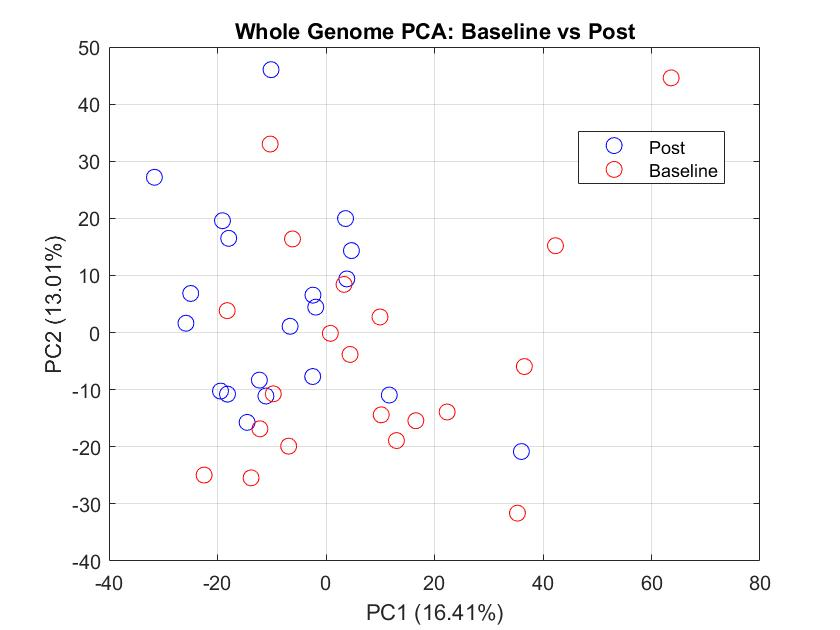
\includegraphics[width=\linewidth]{figures/q1_basevpost.jpg}
    \caption{PCA of baseline vs post-intervention}
    \label{fig:q1_1}
\end{minipage}
\hfill
\begin{minipage}{0.48\linewidth}
    \centering
    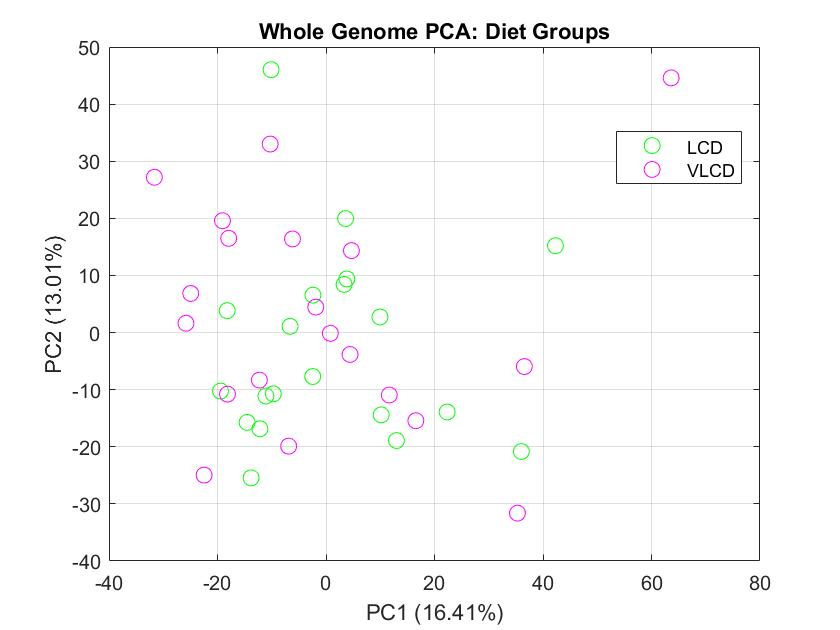
\includegraphics[width=\linewidth]{figures/q1_diet.jpg}
    \caption{PCA of LCD vs VLCD}
    \label{fig:q1_2}
\end{minipage}
\end{figure}

\begin{figure}[H]
\centering

\begin{minipage}{0.48\linewidth}
    \centering
    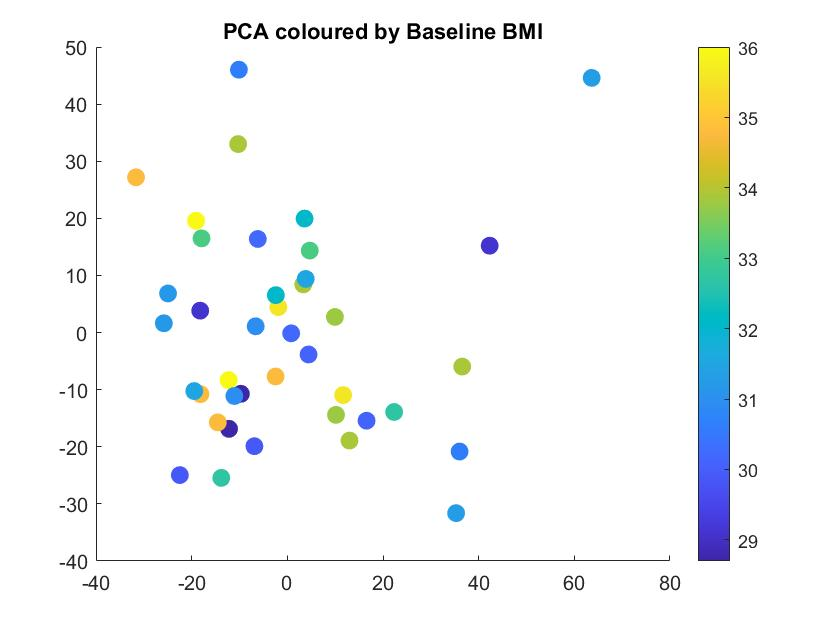
\includegraphics[width=\linewidth]{figures/q1_bmi.jpg}
    \caption{PCA of BMI}
    \label{fig:q1_3}
\end{minipage}
\hfill
\begin{minipage}{0.48\linewidth}
    \centering
    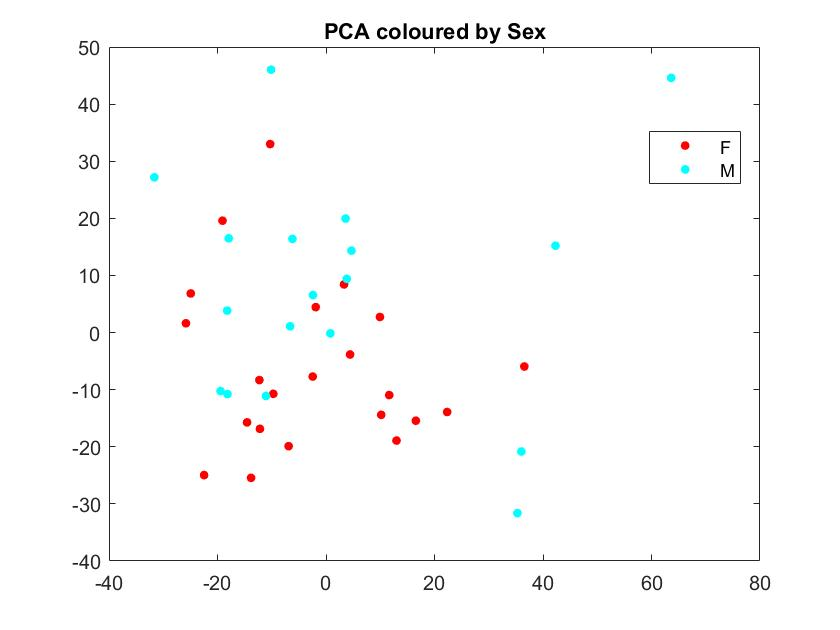
\includegraphics[width=\linewidth]{figures/q1_sex.jpg}
    \caption{PCA of sex}
    \label{fig:q1_4}
\end{minipage}
\end{figure}
% Placeholder for teammate's content:
% - Explained variance in PC1 and PC2
% - Scatter plot coloured by diet group, before/after
% - Discussion of clusters and driving factors

% ============================================================================
\section{Question 2: Context-Specific Models Generation from Recon3D}
\label{sec:q2}
In total of 20 context-specific metabolic models were generated using the iMAT algorithm with the Recon3D genome-scale metabolic model and the baseline adipose tissue gene expression data. Gene expression values were first mapped to metabolic reactions using the gene-protein-reaction (GPR) rules in Recon3D. This mapping assigns an expression score to each reaction based on the associated genes.

\subsection{Characteristics and boundaries choice of iMAT}
The iMAT algorithm classifies reactions as highly expressed, intermediate and lowly expressed using expression thresholds. It then solves a mixed-integer linear programming problem that maximizes flux through highly expressed reactions while minimizing flux through lowly expressed reactions, subject to the stoichiometric constraints of the metabolic network. In this section, the 25th and 75th percentiles of the reaction expression distribution were used as lower and upper threshold. These thresholds adapt to the data distribution and avoid arbitrary fixed cut-offs.

An advantage of iMAT is that is does not require a predefined metabolic objective function, making it suitable for tissue-specific model generation when the biological objective is unclear. However, the results depend on the chosen thresholds and assume that gene expression correlates with metabolic activity.

\subsection{Comparison between different reconstruction methods}
Compared to other reconstruction methods, GIMME requires a predefined metabolic objective and removes reactions inconsistent with gene expression while maintaining that objective. E-Flux constrains reaction flux bounds directly using gene expression values rather than selecting reactions. FASTCORE requires a predefined set of core reactions and builds the smallest consistent network containing them. In contrast, iMAT balances the activation of highly expressed reactions and suppression of lowly expressed reactions, making it suitable for generating individualized models without requiring prior knowledge of core metabolic functions.

% Placeholder for teammate's content:
% - Description of iMAT algorithm
% - Hyperparameter choices (thresholds)
% - Pros/cons vs GIMME, E-Flux, FASTCORE
% - 20 baseline models generated

% ============================================================================
\section{Question 3: Context-Specific Models from Foguet Adipocyte Reconstruction}
\label{sec:q3}
\subsection{Comparison between Recon3D and Foguet reconstruction}
Using iMAT, context-specific models derived from Recon3D contained approximately 4327 to 4607 reactions and 2886 to 3135 metabolites across participants, whereas Fouget-derived adipocyte models contained only 485 to 514 reactions and 409 to 435 metabolites. This nearly ten-fold difference in reaction count reflects the fundamental distinction between the two draft reconstructions. Recon3D is a comprehensive, multi-tissue human metabolic network, and even after pruning it retains a broad metabolic scope. In contrast, the Fouget model is already curated for adipocyte metabolism, resulting in substantially smaller and reconstructions that focus more on the tissue.

\subsection{Model characteristics derived from different reconstruction methods}
The Recon3D models therefore preserve a wider range of metabolic capabilities, potentially including pathways not physiologically relevant to adipose tissue. Fouget-derived models provide greater tissue specificity and improved interpretability for adipocyte metabolism, but at the cost of reduced global metabolic coverage. Thus, the choice of draft reconstruction significantly influences the structural size, metabolic scope, and interpretability of the individualized context-specific models.

% Placeholder for teammate's content:
% - Comparison of Recon3D vs Foguet-derived models
% - Differences in model size, reaction coverage

% ============================================================================
\section{Question 4: Comparing Baseline Context-Specific Models}
\label{sec:q4}

\subsection{Model Selection and Overview}

For this analysis, we compared context-specific models generated from both the Recon3D generic reconstruction and the Foguet adipocyte model. We selected the \textbf{Foguet adipocyte model} for the subsequent analysis because it provides greater tissue specificity for adipose metabolism, yielding models of interpretable size (approximately 470--550 reactions) rather than the much larger Recon3D-derived models (over 4000 reactions) that retain many pathways irrelevant to adipocyte function.

The 20 baseline context-specific models were generated using iMAT (Section~\ref{sec:q2}), where each model represents the predicted active metabolic network of an individual's adipose tissue at baseline.

\subsection{Reaction and Metabolite Counts}

Table~\ref{tab:model_sizes} summarises the number of reactions and metabolites in each context-specific model. Across the 20 baseline models, the mean number of reactions was $498.8 \pm 22.0$, ranging from 469 to 550. The total number of unique reactions across all models was 805. Model sizes were comparable between diet groups: the VLCD group averaged $499.5$ reactions and the LCD group $498.0$ reactions, which is expected since both groups share the same pre-intervention condition. The largest model (P25, VLCD, 550 reactions) and smallest model (P06, LCD, 469 reactions) differ by approximately 17\%, reflecting moderate inter-individual variability in predicted active metabolic networks.

\begin{table}[H]
\centering
\caption{Reaction and metabolite counts for each baseline context-specific model.}
\label{tab:model_sizes}
\begin{tabular}{lcccl}
\toprule
\textbf{Participant} & \textbf{Diet} & \textbf{Reactions} & \textbf{Metabolites} & \textbf{Sex} \\
\midrule
P01 & VLCD & 492 & 412 & F \\
P02 & VLCD & 503 & 426 & F \\
P03 & VLCD & 496 & 417 & M \\
P04 & VLCD & 491 & 410 & F \\
P05 & VLCD & 501 & 418 & M \\
P06 & LCD  & 469 & 396 & F \\
P08 & LCD  & 493 & 411 & F \\
P09 & LCD  & 505 & 416 & F \\
P10 & LCD  & 493 & 415 & F \\
P11 & LCD  & 526 & 449 & M \\
P12 & VLCD & 494 & 411 & F \\
P13 & LCD  & 502 & 420 & F \\
P14 & LCD  & 479 & 399 & M \\
P19 & LCD  & 520 & 431 & F \\
P20 & LCD  & 508 & 430 & M \\
P21 & VLCD & 470 & 396 & F \\
P22 & VLCD & 484 & 405 & M \\
P23 & LCD  & 485 & 409 & M \\
P25 & VLCD & 550 & 462 & M \\
P26 & VLCD & 514 & 435 & M \\
\bottomrule
\end{tabular}
\end{table}

\subsection{Jaccard Similarity Analysis}

To compare the structural similarity of the context-specific models, we computed the pairwise Jaccard similarity index based on the sets of active reactions:
\begin{equation}
    J(A, B) = \frac{|A \cap B|}{|A \cup B|}
\label{eq:jaccard}
\end{equation}
where $A$ and $B$ are the reaction sets of two models. $J = 1$ indicates identical reaction sets, $J = 0$ no overlap.

The mean pairwise Jaccard similarity was $0.7404 \pm 0.0479$. Within-group similarities were comparable to between-group similarities (VLCD: $0.7387 \pm 0.0380$, LCD: $0.7412 \pm 0.0500$, between: $0.7409 \pm 0.0512$), confirming that the diet assignment does not drive structural differences at baseline. This is expected, since both groups share the same pre-intervention condition and were randomised to diet groups only after the baseline biopsy. The core reaction analysis identified 323 core reactions in the VLCD group and 320 in the LCD group, with 289 reactions shared between both groups and only 34 and 31 unique to VLCD and LCD respectively.

\begin{figure}[H]
\centering
\includefigure[width=0.85\textwidth]{figures/Q4_clustered_jaccard_fouget.png}
\caption{Clustered Jaccard similarity heatmap of the 20 baseline context-specific models. Rows and columns ordered by hierarchical clustering (average linkage). The tightest cluster groups P04, P14, and P10 (Jaccard distance $\approx 0.14$), which includes both VLCD and LCD participants, indicating that inter-individual metabolic similarity is not driven by diet assignment.}
\label{fig:jaccard_heatmap}
\end{figure}

\begin{figure}[H]
\centering
\includefigure[width=0.7\textwidth]{figures/Q4_dendrogram_fouget.png}
\caption{Dendrogram from hierarchical clustering on Jaccard distance (average linkage). The deepest branch separates a cluster of outliers (P11, P08, P23, P21) from the remaining participants. Within the main group, VLCD and LCD participants are interleaved, confirming no diet-driven structural clustering at baseline.}
\label{fig:jaccard_dendro}
\end{figure}

\subsection{Multidimensional Scaling}

To visualise the Jaccard distances in two dimensions, we applied classical multidimensional scaling (MDS). Figure~\ref{fig:jaccard_mds} shows the projection coloured by diet group, sex, and baseline BMI.

\begin{figure}[H]
\centering
\includefigure[width=\textwidth]{figures/Q4_MDS_jaccard_fouget.png}
\caption{MDS projection of Jaccard distances, coloured by (a)~diet group, (b)~sex, (c)~baseline BMI. VLCD and LCD samples are intermingled with no visible separation. Males (P05, P20, P21) tend to occupy the lower portion of MDS2, suggesting a weak sex-related trend. No clear BMI gradient is apparent along either axis.}
\label{fig:jaccard_mds}
\end{figure}

\subsection{Comparison with Recon3D vs Foguet Reconstructions}

As discussed in Section~\ref{sec:q3}, Recon3D-derived models contain approximately 4300--4600 reactions, whereas Foguet-derived models contain 469--550 reactions. The nearly ten-fold size difference means that Jaccard similarities are generally higher for Recon3D models (more shared reactions in a larger network), while Foguet models amplify inter-individual differences in tissue-relevant pathways. The Foguet models are therefore better suited for detecting subtle metabolic differences between individuals in adipose-specific metabolism, whereas Recon3D models retain pathways that are unlikely to be active in adipocytes, diluting the biological signal.

\subsection{Comparison with Gene Expression PCA (Question 1)}

Consistent with the PCA results from Question~1, the Jaccard similarity analysis does not reveal diet-driven clustering at baseline. Both analyses show that inter-individual variability dominates over any group-level effect. However, the MDS projection of Jaccard distances shows a weak tendency for some male participants to cluster separately, which was less visible in the PCA. This difference arises because PCA captures global transcriptomic variance dominated by high-variance genes, while Jaccard similarity reflects the binary structure of the metabolic network, which acts as a nonlinear filter that amplifies pathway-level differences rather than individual gene expression changes.


% ============================================================================
\section{Question 5: Flux Balance Analysis and Cosine Similarity}
\label{sec:q5}

\subsection{Constraint Application}

Before running FBA, we verified the physiological constraints already present in each context-specific model. The Foguet adipocyte model is a manually curated, tissue-specific reconstruction whose exchange reaction bounds already reflect the metabolic environment of subcutaneous adipose tissue. These bounds encode which metabolites the tissue can take up from the bloodstream (e.g., glucose, fatty acids, amino acids, oxygen) and which it secretes (e.g., lactate, glycerol, CO$_2$).

Since iMAT only determines which reactions are active by removing reactions inconsistent with gene expression, it preserves the original exchange reaction bounds from the parent model. The context-specific models therefore already carry physiologically appropriate constraints. Inspection of the exchange reactions in a representative model (P01) confirmed 91 exchange reactions with 16 uptake-only, 13 secretion-only, and 62 bidirectional reactions, with bounds consistent with known adipose tissue physiology (e.g., glucose uptake capped at $\approx 4.8$ mmol/gDW/h, oxygen uptake at $\approx 1.8$ mmol/gDW/h, amino acid uptake at $\leq 0.1$ mmol/gDW/h).

We adopted the existing curated bounds without modification, rather than zeroing all exchanges and selectively re-opening them, because the Foguet bounds are literature-derived and tissue-specific, and overriding them would risk missing essential cofactors or metabolites and causing artificial infeasibility.

\subsection{Objective Function}

We selected \textbf{ATP maintenance demand (ATPM)} as the objective function, maximising the rate of non-growth-associated ATP hydrolysis. This choice is motivated by:

\begin{itemize}[leftmargin=*]
    \item Adipose tissue is \textit{non-proliferating} in adults; a biomass objective (cell growth) is inappropriate.
    \item ATPM captures basal energy expenditure for cellular housekeeping: ion gradients, protein turnover, and membrane integrity.
    \item It provides a physiologically interpretable measure of metabolic capacity.
\end{itemize}

An alternative would be parsimonious FBA (minimising total flux), which identifies the most efficient flux distribution but does not correspond to a specific biological objective.

\subsection{FBA Results}

FBA yielded feasible solutions for 19/20 models. The model for P11 (LCD) was infeasible, likely due to missing exchange reactions required to satisfy the ATP maintenance demand under the applied constraints. The mean objective value (ATPM flux) across feasible models was $13.98 \pm 1.92$ mmol/gDW/h. Objective values clustered around two levels: approximately 12.5 and 15.6 mmol/gDW/h (Figure~\ref{fig:obj_values}), with one outlier at 9.5 (P23). This bimodal pattern suggests that the presence or absence of a small number of key reactions (e.g., in oxidative phosphorylation or the TCA cycle) creates discrete levels of ATP production capacity rather than a continuous distribution.

\begin{figure}[H]
\centering
\includefigure[width=0.7\textwidth]{figures/Q5_objective_values_fouget.png}
\caption{FBA objective values (ATPM flux) for each baseline model, coloured by diet group. VLCD is the orange one, LCD the blue one.}
\label{fig:obj_values}
\end{figure}

\subsection{Cosine Similarity of Flux Distributions}
To compare predicted flux distributions, we computed pairwise cosine similarity:
\begin{equation}
    \cos(\mathbf{v}_A, \mathbf{v}_B) = \frac{\mathbf{v}_A \cdot \mathbf{v}_B}{\|\mathbf{v}_A\| \, \|\mathbf{v}_B\|}
\label{eq:cosine}
\end{equation}
where $\mathbf{v}_A, \mathbf{v}_B$ are flux vectors aligned to a common reaction space (zero flux for absent reactions). Reactions with zero flux across all models were excluded.

We chose covariance similarity because to identify the underlying metabolic signatures within our high-dimensional dataset, we utilized cosine-based metrics for pattern interpolation, in fact, cosine similarity prioritizes the stoichiometric orientation and relative distribution of metabolic pathways, guaranteeing that this approach effectively normalizes for varying metabolic scales while highlighting conserved flux profiles and regulatory shifts across different conditions.

The mean cosine similarity was $0.6292 \pm 0.0951$. Within-group similarity (VLCD: $0.6194 \pm 0.1040$, LCD: $0.6251 \pm 0.0968$) was comparable to between-group similarity ($0.6358 \pm 0.0901$). The cosine similarities are notably lower than the Jaccard similarities from Q4 ($\approx 0.74$), indicating that although models share a large fraction of their reaction sets, the predicted flux distributions differ substantially across individuals. This is consistent with the observation that FBA solutions are sensitive to subtle differences in network topology and constraint values, even when the overall structure is similar.

\begin{figure}[H]
\centering
\includefigure[width=0.85\textwidth]{figures/Q5_clustered_cosine_fouget.png}
\caption{Clustered cosine similarity heatmap of FBA flux distributions for baseline models.}
\label{fig:cosine_heatmap}
\end{figure}

\begin{figure}[H]
\centering
\includefigure[width=\textwidth]{figures/Q5_MDS_cosine_fouget.png}
\caption{MDS projection of cosine distances, coloured by (a)~diet group, (b)~sex, (c)~baseline BMI. Diet groups remain intermingled. A loose cluster of outliers (P13, P23, P01) appears in the upper portion of MDS2, driven by lower ATP production and distinct flux patterns. No clear BMI gradient is observed.}
\label{fig:cosine_mds}
\end{figure}

\subsection{Comparison Across Methods}

Table~\ref{tab:comparison} summarises clustering tendencies across the three levels of analysis.

\begin{table}[H]
\centering
\caption{Clustering patterns across analysis methods.}
\label{tab:comparison}
\begin{tabular}{lccc}
\toprule
\textbf{Feature} & \textbf{PCA (Q1)} & \textbf{Jaccard (Q4)} & \textbf{Cosine (Q5)} \\
\midrule
Diet group clusters    & NO & NO & NO \\
Sex-driven clusters    & NO & Weak & NO \\
BMI gradient visible   & NO & NO & NO \\
\bottomrule
\end{tabular}
\end{table}

Across all three levels of analysis, diet group assignment does not produce visible clustering at baseline. This is expected because both groups were measured before any dietary intervention, and randomisation should produce comparable groups. The three methods capture complementary aspects of the data: PCA reflects global transcriptomic variation dominated by the highest-variance genes; Jaccard similarity captures the binary network structure (active vs inactive reactions), which is robust to noise but insensitive to quantitative differences; and cosine similarity on flux distributions captures the functional metabolic state, shaped by both network topology and physiological constraints. The weak sex-related trend visible in the Jaccard MDS but absent in PCA and cosine MDS suggests that sex influences which reactions are retained by iMAT, but this structural difference does not translate into large functional (flux-level) differences under the applied constraints.


% ============================================================================
\section{Question 6: Post-Intervention Analysis}
\label{sec:q6}

\subsection{FBA Analysis}% Gabriele part

Flux balance analysis was performed on both baseline and post-intervention context-specific models using ATP maintenance demand (\rxn{Adipocytes\_DM\_atp\_c}) as the objective function, consistent with the approach in Section~\ref{sec:q5}. Exchange reaction bounds were taken directly from the Foguet model curation without additional overrides.

Of the 20 baseline models, 19 yielded feasible FBA solutions (P11 was infeasible). Among the post-intervention models, 19 were feasible (P23 was infeasible). In total, 18 participants had feasible solutions at both time points and were retained for paired comparison.

Baseline ATP production ranged from 9.54 (P23) to 15.70 (P03) mmol/gDW/h, with a mean of $13.98 \pm 1.92$. Post-intervention values ranged from 9.50 (P11) to 15.69 (P13), with a mean of $14.01 \pm 2.24$. The overall mean ATP flux remained stable across the intervention, although individual participants showed notable shifts: for example, P01 increased from 12.48 to 14.93 mmol/gDW/h, while P14 decreased from 12.50 to 9.57 mmol/gDW/h.

To identify reactions with statistically significant flux changes between baseline and post-intervention, we applied the Wilcoxon signed-rank test (paired, $p < 0.05$) within each diet group. In the VLCD group, two reactions showed significant changes: \rxn{Adipocytes\_EX\_ser\_Le\_bc} (serine exchange, mean change $-0.012$, $p = 0.031$) and \rxn{Adipocytes\_GHMT2r} (glycine hydroxymethyltransferase, mean change $+0.009$, $p = 0.031$). These two reactions are metabolically linked, as serine is converted to glycine by GHMT2r, suggesting a coordinated shift in one-carbon metabolism under very low caloric restriction. In the LCD group, one reaction reached significance: \rxn{Adipocytes\_THRGLYexR} (mean change $-250.0$, $p = 0.031$). The large magnitude of this change likely reflects a binary switch in pathway activity rather than a gradual quantitative shift. No reactions were significant in both diet groups, indicating that the two interventions produce partially distinct metabolic responses at the flux level.

\subsection{Reactions comparison between baseline and post-intervention models}
Context-specific metabolic models were generated for both baseline and post-intervention samples using the iMAT algorithm applied to Fouget adipocyte model. Flux balance analysis was then performed on each model using ATP maintenance (ATPM) as the objective function to represent cellular energy demand.

To evaluate how strongly metabolism changed after the intervention, cosine similarity was computed between the baseline and post-intervention flux distributions for each participant. As shown in Figure~\ref{fig:q6_1}, most cosine similarity values range between approximately 0.5 and 0.8 (note that P11 and P23 are infeasible), indicating that although many reactions remain similar, substantial metabolic changes occur after the dietary intervention.

Structural differences between the metabolic networks were also examined by comparing the reactions present in the baseline and post-intervention models. The results show substantial remodeling of the metablic networks. In the VLCD group, 439 reactions were newly activated after the intervention and 408 reactions were lost. Similarly, in the LCD group, 431 reactions were gained and 392 reactions were lost.

Several reactions appeared repeatedly among the newly activated reactions across participants. Examples like \rxn{Adipocytes\_C180CPT2}, \rxn{Adipocytes\_C180CRNt} and \rxn{Adipocytes\_FAOXC180}, which are associated with mitochondrial fatty acid transport and $\beta$-oxidation. Other reactions such as \rxn{Adipocytes\_ICDHy} belong to the tricarboxylic acid (TCA), indicating increased mitochondrial metabolic activity.

The overall structural similarity between baseline and post-intervention models was further evaluated using the Jaccard similarity coefficient, shown in Figure~\ref{fig:q6_2}. The values generally remain relatively high, around 0.65 to 0.85, suggesting that most reactions remain shared between the models while a smaller subset of reactions accounts for the metabolic adaptation.
\begin{figure}[H]
\centering

\begin{minipage}{0.48\linewidth}
    \centering
    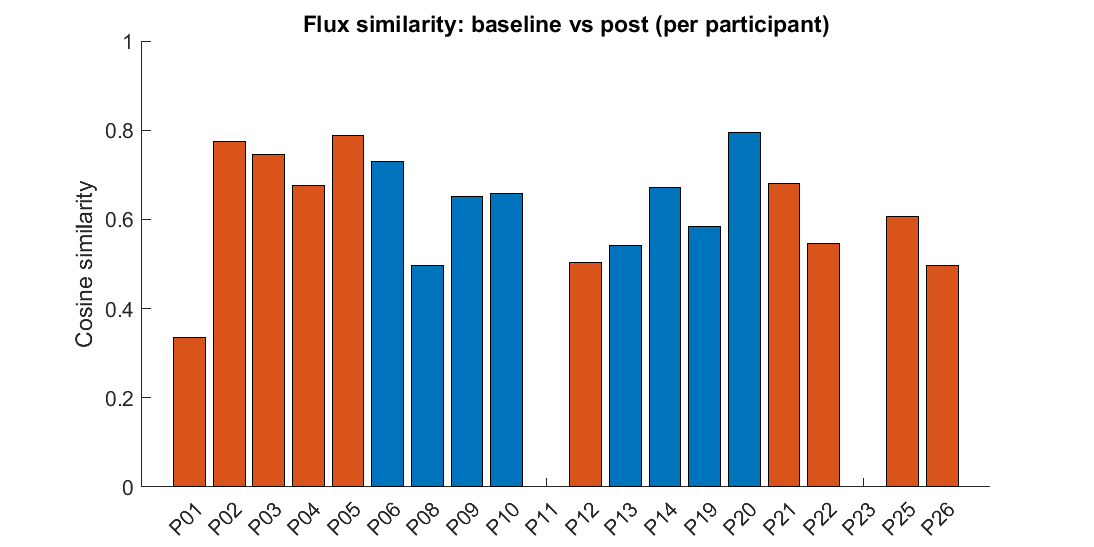
\includegraphics[width=\linewidth]{figures/Q6_cosine_BL_vs_post.png}
    \caption{Cosine similarity between baseline and post-intervention models}
    \label{fig:q6_1}
\end{minipage}
\hfill
\begin{minipage}{0.48\linewidth}
    \centering
    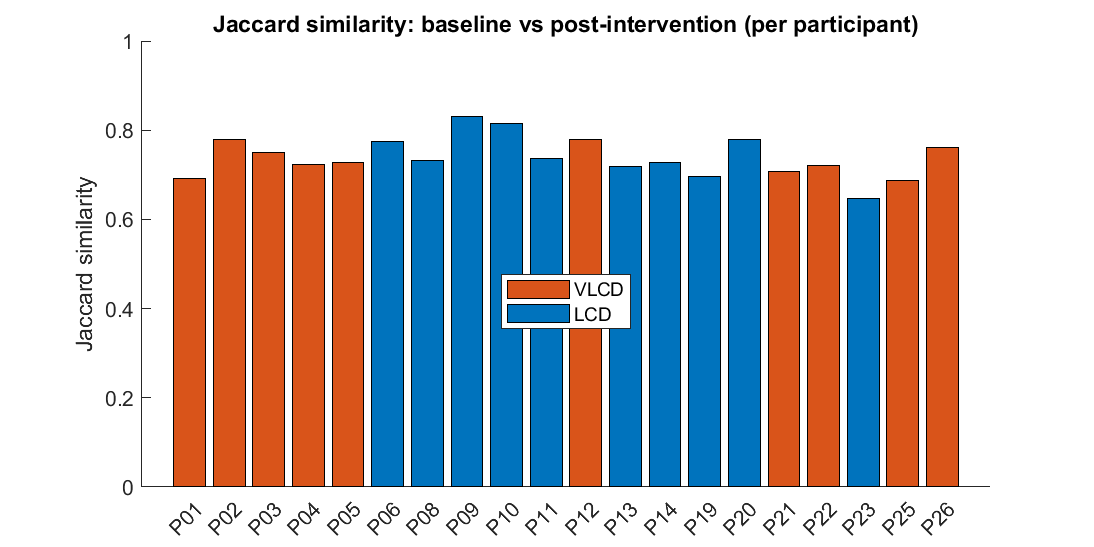
\includegraphics[width=\linewidth]{figures/Q6_jaccard_BL_vs_post.png}
    \caption{Jaccard similarity between baseline and post-intervention models }
    \label{fig:q6_2}
\end{minipage}
\end{figure}

\subsection{Comparison betwwen LCD and VLCD diet groups}
Although both diets produced large metabolic changes, the majority of newly activated reactions were shared between the two groups. A total of 317 reactions were gained in both diets, while 122 reactions were unique to the VLCD group and 114 reactions were unique to the LCD group.

Hierarchical clustering of all baseline and post-intervention models, shown in Figure~\ref{fig:q6_3}, provides an overview of the relationships between metabolic reconstructions. The clustering indicates that several post-intervention models group closely with their corresponding baseline models, suggesting that individual-specific metabolic characteristics remain partially preserved after the intervention.

Despite these similarities, clear metabolic shifts are still visible across participants. The model size comparison shown in Figure~\ref{fig:q6_4} demonstrates moderate changes in the number of reactions and metabolites between baseline and post-intervention networks. These differences reflect the activation or removal of specific metabolic pathways in response to the dietary intervention.
\begin{figure}[H]
\centering

\begin{minipage}{0.48\linewidth}
    \centering
    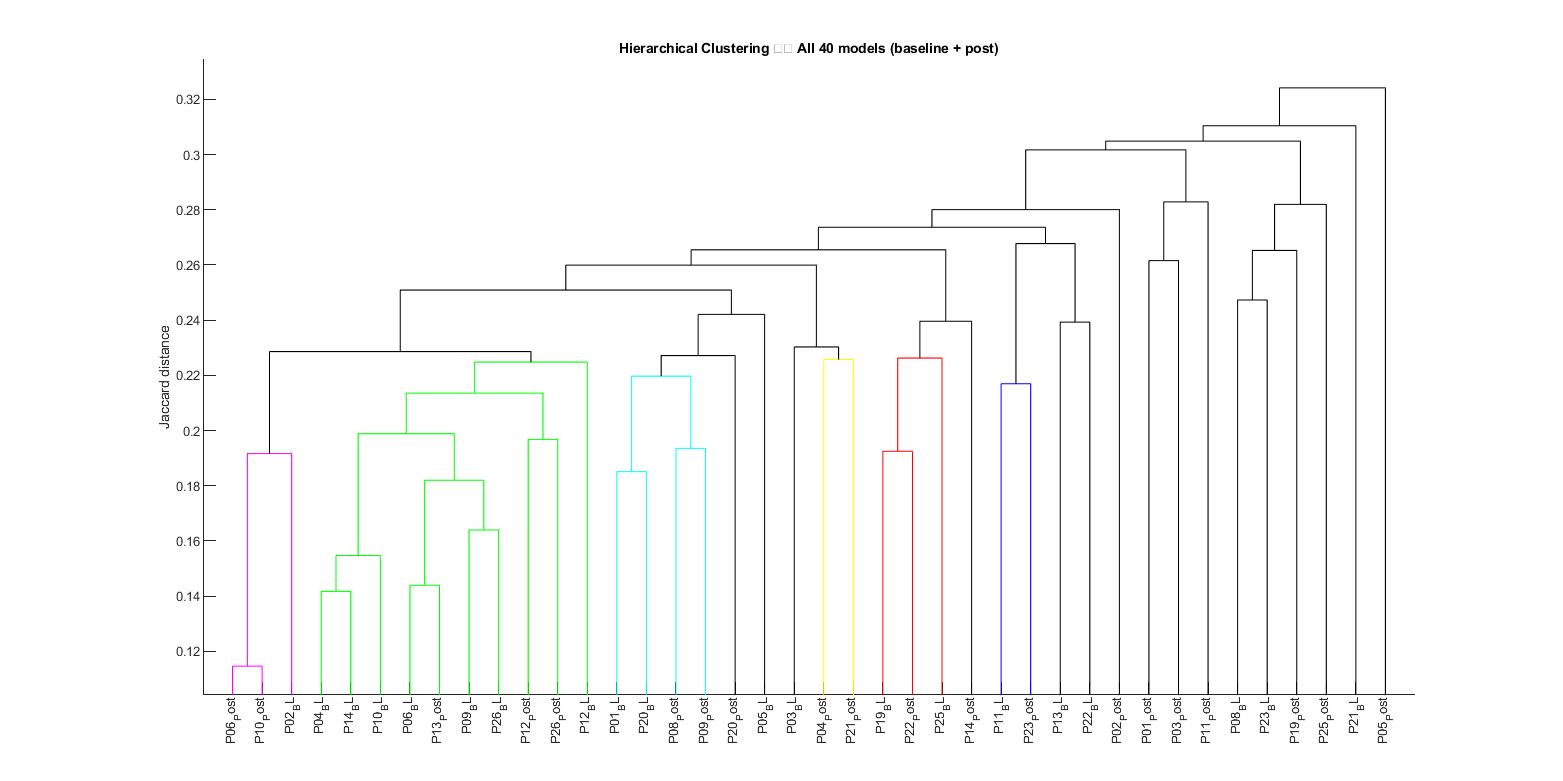
\includegraphics[height=4.2cm]{figures/Q6_dendrogram_40models.png}
    \caption{Dendrogram of baseline and post-intervention models}
    \label{fig:q6_3}
\end{minipage}
\hfill
\begin{minipage}{0.48\linewidth}
    \centering
    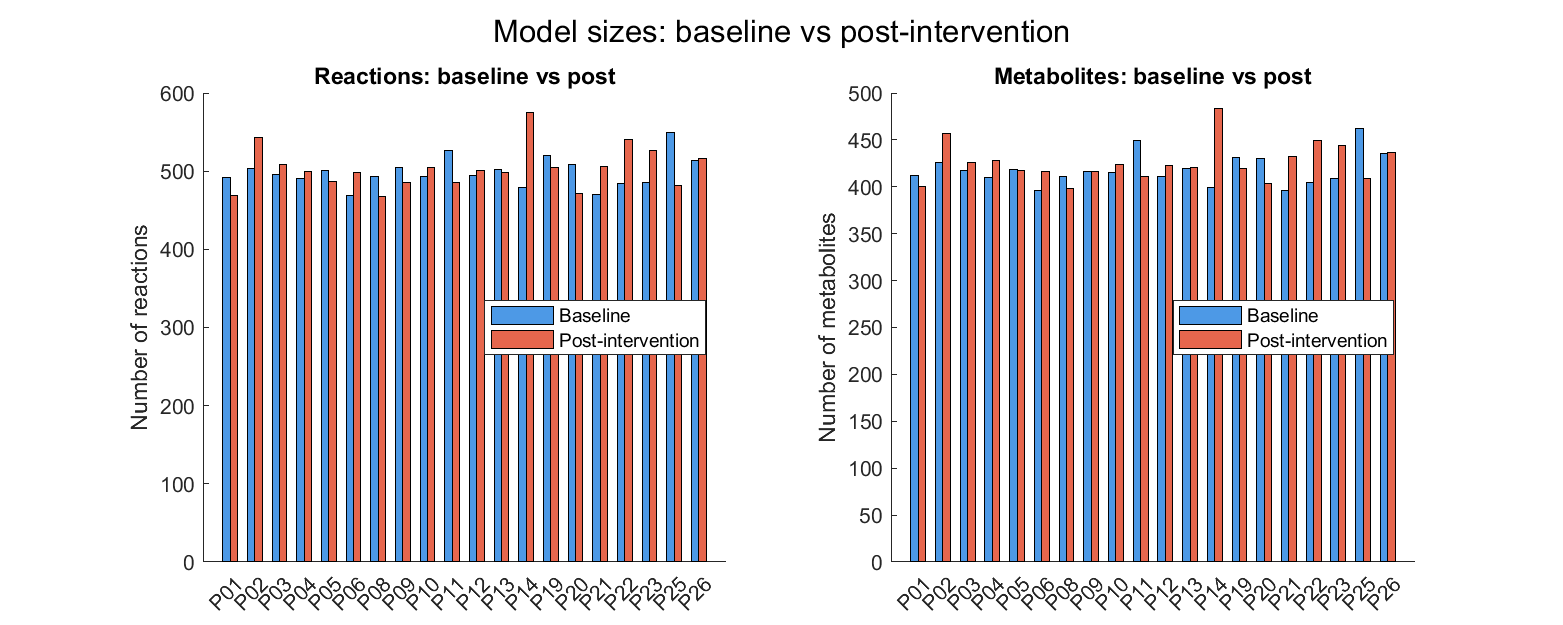
\includegraphics[height=3.8cm]{figures/Q6_model_size_comparison.png}
    \caption{Model size comparison between baseline and post-intervention models }
    \label{fig:q6_4}
\end{minipage}
\end{figure}

\subsection{Biological interpretation and relation to the literature}
The reactions identified in the post-intervention models correspond to pathways known to be involved in adipose tissue adaptation during weight loss. In particular, reactions associated with fatty acid $\beta$-oxidation, mitochondrial energy metabolism, and the TCA cycle were frequently observed among the newly activated reactions.

Increased activity of fatty acid oxidation pathways indicates enhanced lipid utilization, which is expected during caloric restriction when stored triglycerides are mobilized for energy production. The presence of additional TCA cycle reactions further suggests increased mitochondrial oxidative metabolism.

The metabolic consequences of these changes are reflected in the predicted ATP production capacity of the models. As shown in Figure~\ref{fig:q6_5}, several post-intervention models exhibit slightly higher ATP flux values compared to baseline models, indicating increased energetic efficiency and oxidative metabolism.
\begin{figure}[H]
    \centering
    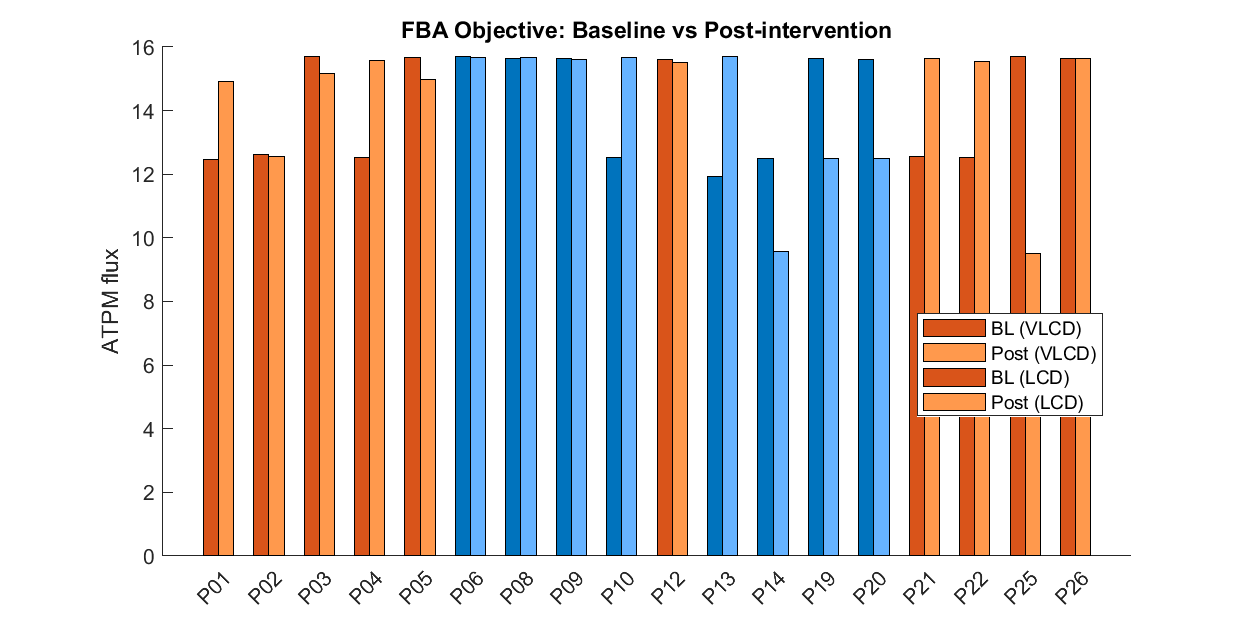
\includegraphics[width=0.5\linewidth]{figures/Q6_objective_BL_vs_post.png}
    \caption{ATP flux values of baseline and post-intervention models}
    \label{fig:q6_5}
\end{figure}

The predicted metabolic fluxes show partial agreement with the gene expression results reported by Vink et al., who observed stronger upregulation of genes related to mitochondrial function, immunity/inflammation and angiogenesis in the VLCD group compared with the LCD group. In the flux analysis, several reactions associated with mitochondrial metabolism, including the fatty acid $\beta$-oxidation and TCA cycle reactions, were frequently activated in the post-intervention models. These pathways contribute directly to mitochondrial oxidative metabolism and ATP production, indicating increased mitochondrial activity during caloric restriction. This observation is consistent with the upregulation of mitochondrial gene sets reported in the original study.

However, pathways related to immunity or angiogenesis were not clearly reflected in the predicted metabolic fluxes. This discrepancy is expected because genome-scale metabolic models represent metabolic reactions and energy metabolism, whereas immune signalling and angiogenic processes are primarily regulated through signalling and transcriptional networks that are not explicitly captured in constraint-based metabolic models. Therefore, the flux analysis supports the mitochondrial component of the transcriptional findings, while providing only indirect evidence for the broader biological processes described in the original study.

% ============================================================================
\section{Discussion}
\label{sec:discussion}

This assignment applied genome-scale metabolic modelling to analyze adipose tissue metabolism under caloric restriction using transcriptomic data. The PCA results indicated that the largest sources of variation in gene expression are driven primarily by differences between individuals rather than diet group or intervention status. Consistent with this observation, the context-specific metabolic models generated using iMAT showed high structural similarity at baseline and no clustering according to diet group.

Despite the similar network structures, flux balance analysis revealed greater variability in predicted metabolic flux distributions between individuals. This indicates that relatively small structural differences in the metabolic network can lead to distinct functional metabolic states. Post-intervention comparisons suggested metabolic remodeling in pathways related to fatty acid oxidation and mitochondrial energy metabolism, which is consistent with increased lipid utilization during caloric restriction.

% ============================================================================
\section{Conclusion}
\label{sec:conclusion}

In this assignment, context-specific adipose tissue metabolic models were generated from transcriptomic data using the iMAT algorithm and analyzed using structural similarity measures and flux balance analysis. The results show that baseline metabolic networks are largely similar across participants, while predicted metabolic fluxes vary more substantially between individuals.

After the dietary intervention, several metabolic pathways associated with fatty acid oxidation and mitochondrial energy metabolism were activated, reflecting metabolic adaptation to caloric restriction. Overall, this analysis demonstrates how genome-scale metabolic modelling can be used to integrate transcriptomic data and investigate metabolic responses to dietary interventions in human adipose tissue.

% ============================================================================
% REFERENCES
% ============================================================================
\bibliographystyle{plainnat}
% \bibliography{references}    % uncomment if using a .bib file

% Manual references (if not using BibTeX):
\begin{thebibliography}{9}

\bibitem[Vink et~al.(2017)]{vink2017}
R.~G. Vink, N.~J. Roumans, L.~A.~J. Arkenbosch, E.~C.~M. Mariman, and M.~A. van Baak.
\newblock Adipose tissue gene expression is differentially regulated with different rates of weight loss in overweight and obese humans.
\newblock \textit{International Journal of Obesity}, 41(2):309--316, 2017.

\bibitem[Foguet et~al.(2019)]{foguet2019}
C.~Foguet, Y.~Xu, S.~C.~Burgess, and M.~Cascante.
\newblock Constraint-based metabolic modelling of the human adipocyte.
\newblock 

\bibitem[Thiele et~al.(2013)]{thiele2013}
I.~Thiele, N.~Swainston, R.~M.~T. Fleming, et~al.
\newblock A community-driven global reconstruction of human metabolism.
\newblock \textit{Nature Biotechnology}, 31(5):419--425, 2013.

\bibitem[Brunk et~al.(2018)]{brunk2018}
E.~Brunk, S.~Sahoo, D.~C. Zielinski, et~al.
\newblock Recon3D enables a three-dimensional view of gene variation in human metabolism.
\newblock \textit{Nature Biotechnology}, 36(3):272--281, 2018.

\bibitem[Shlomi et~al.(2008)]{shlomi2008}
T.~Shlomi, M.~N. Cabili, M.~J. Herrgård, B.~Ø. Palsson, and E.~Ruppin.
\newblock Network-based prediction of human tissue-specific metabolism.
\newblock \textit{Nature Biotechnology}, 26(9):1003--1010, 2008.

\bibitem[Orth et~al.(2010)]{orth2010}
J.~D. Orth, I.~Thiele, and B.~Ø. Palsson.
\newblock What is flux balance analysis?
\newblock \textit{Nature Biotechnology}, 28(3):245--248, 2010.

\end{thebibliography}
\end{document}